%% -*- Latex -*- 
%% 
%% chap_1.tex - snake and active contour theory
%% 

\chapter{Snake Fundamentals}
\label{sec:snake-fundamentals}

\section{Snakes, Active Contours and Deformable Models}
\label{sec:snakes-methods}

The names of the methods mentioned in the section title have many
labels or names: Snakes, active contours, and deformable models.  They
all refer to the same basic theory; top-down processing in one step
where an initial contour will converge towards the wanted image parts.
No traditional bottom-up processing in two steps is required to first
to segment interesting image features and then next connect these
segmented features. The ``snakes'' term was originally coined with the
first article on snake by \citet{kass88}. Now deformable models is
generally used while the active contours term is used with object
tracking in images the area of computer vision.

To make the contour of a snake move the contour of the snakes have
internal energies assigned to it while the intensity levels in the
image is referred to as external energy levels. The snake methods will
find an energy equilibrium from which a final contour is extracted. An
example will illustrate the basics of the snake method. A basic snake
method by \citet{xu97a,xu97b} has been modified to obtain the example
on figure~\ref{fig:snake-example-start} (to show a contour at every
five iterations). In the example an image of a black circle with white
background must be extracted. On the left image of
figure~\ref{fig:snake-example-start} the initial contour can be seen
converge towards the black circle on the image. The initial contour
have its corners smoothed by the internal energies while the contour
as an overall is attracted towards the external energy of the black
circle. It is the combined energies that make the contour converge
towards the black parts of the image. The right image of
figure~\ref{fig:snake-example-start} shows the final image with the contour
resting where an energy equilibrium has been found.
\begin{figure}[htbp] \centering
  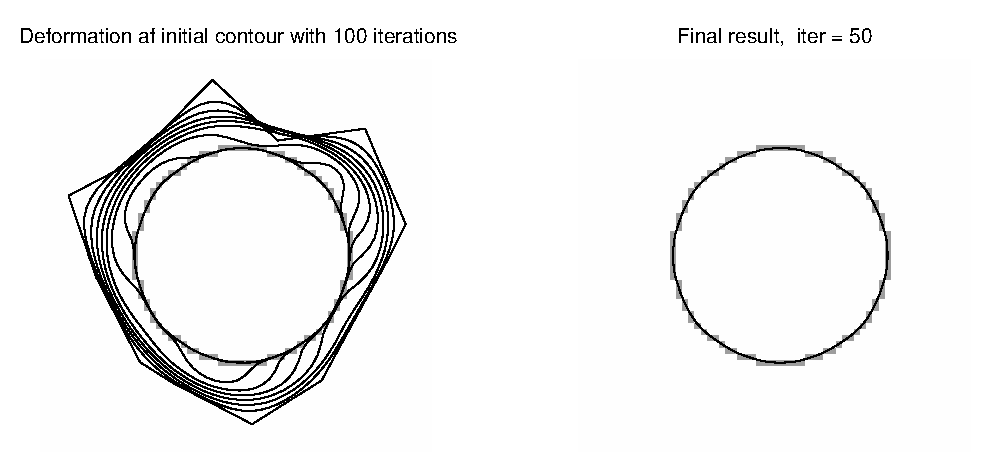
\includegraphics[width=0.8\textwidth]{snake-example-start.eps}
  \caption{Illustration of a snake contour that converges towards on
    an image of a circle. On both images the grey area is the image
    part to extract a contour for. The left images shows initial
    contour and contours for every 5 iterations of the snake method
    for 100 iterations. The right image shows the final result (found at
    iteration number 50).}
  \label{fig:snake-example-start}
\end{figure}

The example was given for a two-dimensional image and contour. The
following sections will present previous work of deformable models. 
A major part of the previous work have been defined for
two-dimensional problems, but may eventually be extended to
three-dimensional deformable models. 

\section{Previous Work}
\label{sec:previous-work}

Active research has been performed in the area of deformable models for
more than ten years, where several variants have been formulated and
several different energy minimization methods have been
introduced. Throughout the years different mathematical notations have
been used in the literature by the different authors. To avoid
confusion the terms used in this report is standardized and will be
in accordance with the article by \citet{kass88}.

This review of previous work will include several articles in
different domains of the segmentation method known as deformable models
or snakes. Usually the deformable model methods are used in a
two-dimensional context, but because of the purpose of this project
the material reviewed must be applicable in a three-dimensional
context. Fortunately to some extent the methods can be used on
three-dimensional data and produce surface models of the data. In
order to present the information properly the review is split into
several sections, each presents an important area of the deformable
model method. There are three distinct areas of snakes:
The representation of the snake, the snake energy function and the
related energy minimization method.

The contour of a snake uses an geometrical representation often
derived from the data and the data dimension. Since the segmentation
of the cerebral vasculature is central to the project focus is needed
on the demands of the representation of the contour. Deformable models
define an energy function which is used in the aim to obtain an
equilibrium of the energy function, and thus segmenting the data.
Obtaining an equilibrium is dependent upon an energy minimization
method in order to reach the energy equilibrium.

\subsection{Snake Representation}
\label{sec:snake-representation}

Several snake representations have been proposed since the
introduction of the snakes method in 1987. The representation of
snakes is central to the behavior of the snake and has been subject to
improvements and new formulations to alter the behavior of the
traditional snake formulation.

The representation of the snake is dependent on the image (or in the
case of this thesis the three-dimensional volume) which the snake
operate upon. Where the image or volume is either two- or
three-dimensional, the representation of the snake has a co-dimension
of one, two or three. Generally the co-dimension of the representation
then determines the model of the extracted object (see
table~\ref{tab:general-models}). It must be mentioned that for a model
with a co-dimension \emph{lesser} than the dimension of image then the
model (referred to as a contour) can be either open or closed. For a
co-dimension of one the open representation is a line and the closed
representation is a circle. For a co-dimension of two (a surface) the
open representation is a plane, the semi-open representation is
cylindrical, and the closed representation is a spherical.
\begin{table}[htbp]
  \centering
  \begin{tabular}[t]{lll}
    \toprule
    \textbf{Co-dimension} & \textbf{2D Model} & \textbf{3D Model}  \\
    \midrule
    One (1D)   &  Line model & Line model    \\
    Two (2D)   &  Mesh model & Surface model \\
    Three (3D) &             & Solid model   \\
    \bottomrule
  \end{tabular}
  \caption{General models for each co-dimension of the snake representation}
  \label{tab:general-models}
\end{table}
Special representation are formulated to model more specific objects
which may be a representation which enables corners in the contours in
the otherwise smooth contours or the modeling of generalized
cylinders.  The extraction will result in a deformed model of the
representation that fits to the image. Formulation of topologically
adaptable snakes enables the representation to adapt to topologically
complex objects. A feature of topological adaptable snakes is that the
model may split into several models in the adaption process. This way
a white object with embedded dark objects may be segmented with the
dark objects omitted, as the contour may merge with itself to adapt to
the topology \citep{mcinerney95,mcinerney97,mcinerney99}.
\begin{figure}[htbp]
  \centering
  \includegraphics{snake-topological-example.eps}
  \caption{Example of a topological complex image to segment.
    The left figure is the image to segment. The right figure is the
    segmented image which topological complex where the snake must
    adapt to three independent contours.}
  \label{fig:snake-topological-example}
\end{figure}

Since this project will extract blood vessels, which are cylinder-like
objects, there have been a focus on generalized cylinders and
cylinder-like objects. Some projects have focused on special cylinder
representations with new energy formulations or energy minimization
methods.  Special representation builds upon the formulations of
general representations and inherits the behavior. A representation is
sought that models the blood vessel in accordance with the demands
stated in section~\ref{sec:aim-study}.

\subsection{Energy Function}
\label{sec:energy-function}

A traditional snake is a continual contour with a parametrized
representation $r(s) = (x(s),y(s)$ where $s$ is defined in the
interval $[0,1]$. The functions $x(s)$ and $y(s)$ are points of the
curve $r$ for all values of $s$.
\begin{figure}[htbp]
  \centering
  \psfrag{x=x(0)}{$\small x=x(0)$}
  \psfrag{x=x(1)}{$x=x(1)$}
  \psfrag{y=y(0)}{$y=y(0)$}
  \psfrag{y=y(1)}{$y=y(1)$}
  \psfrag{(x(s),y(s))}{$(x(s),y(s))$}
  \psfrag{s=0}{$s=0$}
  \psfrag{s=1}{$s=1$}
  \psfrag{x=x(0.5)}{$x=x(0.5)$}
  \psfrag{x=x(0),x(1)}{$x=x(0),x(1)$}
  \psfrag{y=y(0.25)}{$y=y(0.25)$}
  \psfrag{y=y(0.75)}{$y=y(0.75)$}
  \psfrag{y=y(0),y(1)}{$y=y(0),y(1)$}
  \mbox{%
    \subfigure[Open snake curve]%
    {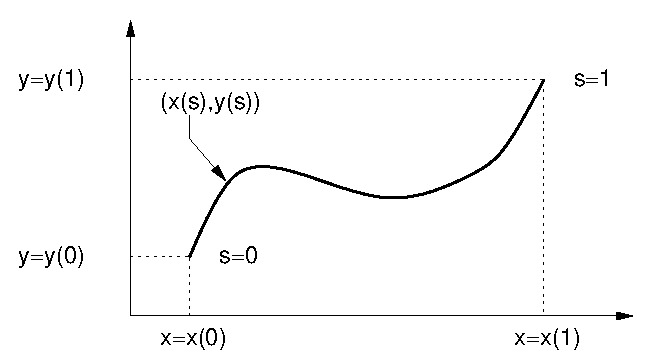
\includegraphics[scale=0.75]{snake-traditional-open.eps}}\quad
    \subfigure[Closed snake curve]%
    {\includegraphics[scale=0.75]{snake-traditional-closed.eps}}}
  \caption{Closed and open snakes curves with the parameter
    representation $C(s)=(x(s),y(s))$}
  \label{fig:snake-traditional-open.eps}
\end{figure}
Snakes are used for segmenting an image, and are dependent upon the
initial location of the contour. The snake method will find its
final representation as a result of an energy function defined with
internal and external energies. The internal energy is defined in
relation to the contour represention only and the external energy is
defined from the image. It is through the minimization of the snake
energy an equilibrium between the internal and the external energies
can be found. Often the minimization is found through an iterative
process which will position the snake contour representation at the
equilibrium between the external and internal energy. Intermediate
steps in the iteration will move the snake towards its final contour
representation.

In the following treatment of the energy terms are presented as in the
traditional two-dimensional work. The terms are extendable to three
dimensions by parameterizing $z = z(s)$, which is an issue considered
when processing volumes instead of images. Different schemes have been
proposed for the internal and external energies and are presented
belonging either to internal energy or external energy. The energy
function $E_{\text{total}}(s)$ is then dependent upon the two energy
terms
\begin{equation}
  \label{eq:energy-total}
  E_{\text{total}}(s) = \int_0^1(E_{\text{internal}}(s)+E_{\text{external}}(s))ds
\end{equation}
which is a summation of the total energy along the arclength $s$ of
the contour.  The integral of the energy terms presented here is
implicitly applied to each of the energy terms presented in the
following sections.  It is the equilibrium between the internal and
external energy that an minimum energy state between the contour
representation and the image is found.

\subsubsection{Internal Energy}
\label{sec:internal-energy}

Internal energy consists of two main energy terms in order to provide
the representation of the contour with several features being
smoothness of the contour, prevent clustering of nodes at the
representation of the contour, and enforcing constraints on the
contour representation. With each new snake formulation of the
internal energy of the minimization of the energy (see
section~\ref{sec:energy-minimization-methods}) new features have been
added. The traditional formulation of the internal energy follows
\begin{equation}
  \label{eq:snake-energy-internal}
  E_{\text{internal}}(s) = 
    E_{\text{tension}}(s) + 
    E_{\text{rigidity}}(s) +
    E_{\text{constraint}}(s)
\end{equation}
The tension and rigidity terms are introduced to enforce a smooth
contour while maintaining an even distribution of nodes on the
representation of the contour. The constraint terms is introduced to
overcome limitations of the tension and rigidity terms.  The tension
energy will for every point on the curve $s(s)$ be defined as
\begin{equation}
  \label{eq:energy-elastic}
  E_{\text{tension}}(s) = \frac{dr(s)}{ds} = \left(\frac{dx(s)}{ds}\right)^2+\left(\frac{dy(s)}{ds}\right)^2
\end{equation}
The tension energy (also referred to as the elastic force) will try to
minimize the tension energy along the contour. The energy is
proportional to the square of the stretching (the distance between
nodes or the first derivative) of the contour representation at a node (see
figure~\ref{fig:internal-energy-tension}) and provide the snake with a
natural tendency to contract.
\begin{figure}[htbp]
  \centering
  \psfrag{E}{$E$}
  \psfrag{y}{$y$}
  \psfrag{dCds}{$\frac{dr}{ds}$}
  \psfrag{x}{$x$}
  \psfrag{si}{$s_i$}
  \psfrag{si-1}{$s_{i-1}$}
  \psfrag{si+1}{$s_{i+1}$}
  \mbox{%
    \subfigure[Tension energy is proportional to stretching of the contour]{\includegraphics{internal-energy-tension-proportional.eps}}\quad%
    \subfigure[Stretch of the contour at a node where the vectors
    indicate the resulting curve]{\includegraphics{internal-energy-tension-stretch-node.eps}}}
  \caption{Illustration of the tension energy}
  \label{fig:internal-energy-tension}
\end{figure}
The rigidity energy (also referred to as stiffness force) is defined
as follows
\begin{equation}
  \label{eq:internal-energy-rigidity}
  E_{\text{rigidity}}(s) 
    = \frac{d^2r(s)}{ds^2} 
    = \left(\frac{d^2x}{ds^2}\right)^2+\left(\frac{d^2y}{ds^2}\right)^2
\end{equation}
Rigidity energy will introduce stiffness to the contour and thereby
minimizing the bending of the contour. The energy is proportional to
the square of the curvature (the second derivative) of the contour
representation at a node (see
figure~\ref{fig:internal-energy-rigidity}) and provide the snake
representation with a smooth contour.
\begin{figure}[htpb]
  \centering
  \psfrag{E}{$E$}
  \psfrag{d2Cds2}{$\frac{d^2r}{ds^2}$}
  \psfrag{y}{$y$}
  \psfrag{x}{$x$}
  \mbox{%
    \subfigure[Rigidity is proportional to the curvature of the contour]{\includegraphics{internal-energy-rigidity-proportional.eps}}\quad%
    \subfigure[Contour with only tension energy applied]{\includegraphics{internal-energy-rigidity-curvature.eps}}\quad%
    \subfigure[Resulting contour with applied energy rigidity]{\includegraphics{internal-energy-rigidity-curvature-result.eps}}}
  \caption{Illustration of rigidity energy}
  \label{fig:internal-energy-rigidity}
\end{figure}
If the snake contour is only applied with the rigidity energy then the
snake will eventually deform to a circle. With both the tension and
rigidity energy defined the internal energy can then be defined with
weights
\begin{equation}
  \label{eq:snake-internal-energy-weights}
  E_{\text{internal}}(s) =
  \omega_{1}\left(\left(\frac{dx(s)}{ds}\right)^2+\left(\frac{dy(s)}{ds}\right)^2\right)
  + \omega_{2}\left(\left(\frac{d^2x}{ds^2}\right)^2+\left(\frac{d^2y}{ds^2}\right)^2\right)
\end{equation}
where the weights $\omega_{1}$ and $\omega_{2}$ are traditionally
referred to as $\alpha$ and $\beta$. It means that
Eq.~(\ref{eq:snake-internal-energy-weights}) is often encountered in
the literature as
\begin{equation}
  \nonumber
  E_{\text{internal}}(s) = \alpha\left(\left(\frac{dx(s)}{ds}\right)^2+\left(\frac{dy(s)}{ds}\right)^2\right) + \beta\left(\left(\frac{d^2x}{ds^2}\right)^2+\left(\frac{d^2y}{ds^2}\right)^2\right)
\end{equation}
By adjusting the weights the snake will change its characteristics and
will perform differently when applied to an image. It is now possible
to adjust the weights to make the contour more elastic than rigid or
more stiff than elastic.  The internal energy terms must be balanced
by the weights $\omega_1$ and $\omega_2$ based upon the wanted
characteristics of the snake, when applied to specific data. Most
applications set $\omega_1$ and $\omega_2$ to be constant along the
contour, but some applications they may be varied to introduce
specific models.

\subsubsection{External Energy}
\label{sec:external-energy}

Segmentation of images with snakes will attract the snake contour
towards interesting features in the image. The external energy will
provide the ability to detect different features of an image, where
the detection is dependent upon different formulations of the external
energy. Because of the different formulations the external energy is
defined as
\begin{equation}
  \label{eq:snake-energy-external}
  E_{\text{external}}(s) = F(x(s),y(s))
\end{equation}
where the function $F$ is formulated to detect the interesting
features. Often $F$ is defined to detect either lines or edges.
\begin{eqnarray*}
  \label{eq:snake-energy-external-lines}
  F_{\text{line}}(x(s),y(s)) &=& +/- I(x(s),y(s)) \\
  \label{eq:snake-energy-external-edges}
  F_{\text{edge}}(x(s),y(s)) &=& +/- \lvert\nabla I(x(s),y(s))\rvert^{2}
\end{eqnarray*}
The sign of the function $F$ decides whether to maximize or minimize
the external energy in order to detect dark or bright features in the
image. The maximization of $E_{\text{external}}$ is the same as
minimizing $-E_{\text{external}}$ (see
figure~\ref{fig:external-energy-sign}).
\begin{figure}[htbp]
  \centering
  \psfrag{E}{$E$}
  \psfrag{x}{$x$}
  \mbox{%
    \subfigure[Positive external energy defined to extract dark image features]{\includegraphics{external-energy-sign-plus.eps}}\quad%
    \subfigure[Negative external energy defined to extract bright image features]{\includegraphics{external-energy-sign-minus.eps}}}
  \caption{Minimizing and maximizing external energy}
  \label{fig:external-energy-sign}
\end{figure}
As a result deformable models are able to find intensity ridges or
valleys of an image, and will move towards those because of the
definition of external energy.

The internal energy is only defined through the representation of a
contour. Internal energies are not in any way related to the image and
the interesting features to segment. Coupling the contour to the image
and make it converge towards the high or low intensities happen
as a result of the definition of the external energy. For external
energies a potential map may be created which attract the
contour. Different approaches have been taken to attract the contour
towards different images features: lines, edges, line ends, etc. Also
the gradient of an image may be computed to and the image may be
convolved with a Gaussian function to have a broader and smoother area
to attract the contour. Other methods includes computing a distance
map or a gradient vector field \citep{xu97a,xu97b}.

The external energy function must be carefully defined in order to let
the contour converge towards the wanted image features. The contour
will normally end up on high (or low) pixels intensities because of
the external energy definition but that may vary depending on the
internal energies. Eventually the equilibrium between external and
internal energies must be decided upon and depends upon the parameters
used with the energy minimization method.


\subsubsection{Constraints}
\label{sec:constraints}

The original paper by \citep{kass88} defines constraints imposed on an
deformable by interactive means. These constraints are the ``volcano''
and the ``spring''. In an interactive context a volcano will move the
contour away from the location of the volcano to avoid unwanted areas
of an image or data and are dependent upon the time of the user
interaction. The opposite of the volcano, the spring, will drag a
specific part of the contour to a location in the image. For some
applications interactive constraints are the flexibility of deformable
models, which will enable semi-automatic segmentation instead of fully
manual. The volcano energy is
\begin{equation}
  \label{eq:energy-volcano}
  E_{\text{volcano}}(s) = \frac{1}{r(s) - r_{\text{volcano}}}
\end{equation}
where the energy will decline from the point $r_{\text{volcano}}$
ie. being repulsive to the contour.
The spring energy is defined
\begin{equation}
  \label{eq:energy-spring}
  E_{\text{spring}}(s) = -k_1(r(s) - r_{\text{spring}})^2
\end{equation}
where $r(s)$ is a point on the deformable model and
$r_{\text{spring}}$ is a point on the image. 

Interactive imposed constraints are different from the interactive
placement of the initial snake. Deformable model methods will from
interactive constraints be dependent on the operator, location of the
constraints and the time of interaction. Depending on the application
this may be acceptable or may not.

Other proposals for energy definitions have been made. \citet{cohen91}
and \citet{cohen93} have proposed the used of inflationary energy
term, a so-called balloon force which inflates the snake contour.
Along the same lines \citet{xu93} defines a pressure force to cancel
the shrinking effect (shrinking is ``encouraged'' by the tension
energy as a soft constraint). The balloon approach has been further
refined by \citet{wang98} and \citet{li99} to address shortcomings of
the balloon force. Instead of the traditional shrinking of the contour
the balloon force will expand the contour by inflation.  The contour
will have to be initialized inside the region of interest, where a
traditional snake must be initialized outside or near the contour to
obtain. The balloon energy is
\begin{equation}
  \label{eq:energy-balloon}
  E_{\text{balloon}}(s) = -k_2 n(s) - k_3 \frac{\nabla I}{\lvert \nabla I \rvert}
\end{equation}
where $n(s)$ is the normal vector of the snake contour and $k_2$ and
$k_3$ is defined to be smaller than the grid size and $k_2$ smaller
than $k_3$ to prevent the contour to inflate past the edges in the image.
The disadvantages with the original inflation energy proposal is that
the inflation energy may be stronger the external energy, thereby
passing the desired edges in images. The later refinements address
these problems by redefining the inflation energy to match the
shrinking  and external energy  \citep{wang98} \citep{li99}.

When defining the snake energy using constraints the energy definition
could be
\begin{equation}
  \nonumber
  E_{\text{total}}(s) = \int^1_0(E_{\text{internal}}(s) + 
                                 E_{\text{external}}(s) +
                                 E_{\text{constraint}}(s) +
                                 E_{\text{balloon}}(s)) ds
\end{equation}
where the internal, external, and constraint energies may consists of
one or several energy terms themselves.

\subsubsection{Special Models}
\label{sec:special-models}


For special snake models there exists snakes definitions which are
better at modeling specific or fixed topologies or are better to adapt
to a broader range of topologies than the ordinary snake
definitions. In the context of this project tube-like structures or
thin elongated structures are sought.


\citet{mcinerney95} and \citet{mcinerney97} has defined a topological
adaptable snake with a general definition that can fit several
applications. The topologically adaptable snake is able to seamlessly
split or join topologically adaptable snake contours with multiple
contour instances that can be created and destroyed. This class of
snakes are used for extraction of objects with complex shapes or
unknown topologies. Opposed to normal explicit parametric contour
representations the topologically adaptable contour are implicit, and
are less convenient in terms of mathematical formulation, shape
analysis and visualization and user interaction \citep{mcinerney95}.


\citet{mogensen99} has defined a tube snake for extracting thin
elongated structures from contour projections of a three-dimensional
area. The snake is defined in a three-dimensional context thus
extending the energy definition to three dimensions. In two areas the
tube snakes differ from ordinary definitions: the fixed topology of a
tube ie. a circular homogenous generalized cylinder (CHGC) and the
definition of external energy based on contour projections, where the
rest of the tube snakes follow traditional energy definition.


The external energy of tube snakes is defined from the contour
projections, where a three-dimensional volume has not been available.
Two different external energy types are defined, $E_{\text{3D}}$ and
$E_{\text{2D}}$, which both have to take each projection image and
each side of the projected cylinder into account. The
three-dimensional energy is defined through magnitude of the gradient
of the contour image
\begin{equation}
  \nonumber
  E_{\text{tube external 3D}}(s) = - \sum^2_{p=1} \sum^2_{j=1} \omega(s) \lvert\nabla I(p,j,s) \rvert^2
\end{equation}
where $p$ is a projection direction and $j$ is left or right side of
projected cylinder on image. With the two-dimensional energy
definition for tube snakes both the gradient magnitude and the
direction of the gradient is used
\begin{equation}
  \nonumber
  E_{\text{tube external 2D}}(s) = - \sum^2_{p=1} \sum^2_{j=1} \omega(s) \lvert q(j,s) \cdot \nabla I(p,j,s)\rvert^2
\end{equation}
where $q(j,s)$ is vector is a normal to the contour projection. When
the local gradient direction $I$ of the external energy is
perpendicular to the normal vector $q$ of the snake contour a good
edge is found.


Where the tube snake place the spine (the center axis of the tube)
under influence of traditional internal energy definition with
internal and external energy, the radius of the cylinder is found by
initially setting the radius to zero and define an inflation energy
(see the balloon energy above). The inflation energy is defined as
\begin{equation}
  \nonumber
  E_{\text{inflate}}(s) = E_{\text{radius}}(s) + E_{\text{expand}}(s) 
\end{equation}
where the expansion energy will inflate the tube to fit a cylinder and
the radius energy will put constraints upon the variation of radius
along the cylinder.
\begin{eqnarray}
  \nonumber
  E_{\text{radius}}(s) &=& \omega_r(s) \left\lvert\frac{dR}{ds}\right\rvert^2 \\
  E_{\text{expand}}(s) &=& \omega_e(s) \frac{1}{t + R(s))^2}
\end{eqnarray}
where $R(s)$ is the radius of the cylinder and $t$ is offset to avoid
singularities initially when radius is set to zero.



\subsection{Energy Minimization Methods}
\label{sec:energy-minimization-methods}

When a snake contour representation and an energy definition has been
settled for the energy minimization must be applied. For some
applications representation and energy definition may limit the
choices of minimization method, but generally any of the different
methods for minimizing the energy can be used. The advantages and
disadvantages of a energy minimization are, due to the nature of the
snake representation combined with the energy minimization methods,
related to the area of application. Often the papers remark only upon
general aspects on their methods and not the applicability in certain
domains.  Several methods have been reviewed which include the
original proposal by \citet{kass88} which use finite difference
methods (FDM), the FEM method improvement by \citet{cohen91} and
\citet{cohen93}, the dynamic programming approach by \citet{amini88}
and \citet{amini90}, the greedy algorithm proposed by
\citet{williams90} and further improved by \citet{yan94} and
\citet{yan97}, B-snakes proposed by \citet{menet90}, geodesic methods
by \citet{lorigo98,caselles97} and geometric minimization method by
\citet{osher88}.


\subsubsection{Finite Difference Method}
\label{sec:finite-differrence-method}

The traditional method for snake energy minimization is the finite
difference method (FDM)
\citep{kass88,waite90,leymarie92,leymarie93,hassanien99}. It is often
used because of the simplicity involved in finding a solution. The FDM
snake consists of $N$ nodes, which defines the contour of the snake.
Energy minimization of FDM is based on Euler-Lagrange equations which
find the energy minimum based on variational calculus. The minimal
solution is found from eq.~(\ref{eq:energy-total}) which must satisfy
the Euler-Lagrange condition
\begin{equation}
  \nonumber
  \frac{d}{ds}E_{r_{s}} - E_{r} = 0
\end{equation}
where $E_{r}$ is the partial derivative of $E$ with respect to $r$ and
$E_{r_{s}}$ is the partial derivative of $E$ with respect to $r_{s}$,
the first derivative of $r$.

From the Euler-Lagrange condition the following equations for each
principal dimension can be derived
\begin{equation}
  \nonumber
  \alpha k_{ss} + \beta k_{ssss} + \frac{\partial
  E_{\text{external}}}{\partial k} = 0
\end{equation}
where $k$ is $x$ and $y$ for two-dimensional data and $x$, $y$, and
$z$ for three-dimensional. By approximation the derivatives can be
computed by finite differences (see
appendix~\ref{sec:difference-derivatives}). The equations can be
written as an $N \times N$ matrix, which is solved iteratively for
each principal dimension. A solution by finite
differences must respect the boundary conditions which is dependent on
the contour representation being open or closed. The closed contour
solves the boundary conditions by wrap-around of the contour
representation so the first points will overlap the last points of the
contour. For open contours the boundary conditions will have to be
computed and often assumptions of the boundary conditions are made
from the fixation of the end points. As a result only the interior of
the contour may alter its position from the FDM method.

Several problems exist with the FDM energy minimization method. It is
only based on the information at the nodes ie. the control points of
the snake. To produce an accurate result the contour must be sampled
by a sufficiently large number of control points to segment fine
details of the contour. Because of the complexity of the solution by
the iterative Euler-method the large number of nodes will increase the
computation time in order to compensate for the needed accuracy.  The
nodes of the contour tend to gather at points in the image which have
a large external energy, as the nodes may move along the contour with
no hard constraints enforced on contour representation
\citep{amini90}. The FDM method uses discretizing of the location of
nodes. As a result a node may oscillate between two locations on the
snake because the minima of the contour is placed between the two
discretized locations.  (see figure \ref{fig:energy-zero-transition})
\citep{cohen91}. The step size for moving a node is proportional to
the external energy which will gives two disadvantages: In areas with
a large external energy the snake will move in large steps sometimes
surpassing the contour to segment and thus never finding a minimum. In
areas with low external energy the snake may nearly not move
\citep{cohen91}.
\begin{figure}[htbp]
  \centering
  \psfrag{f(x)}{$f(x)$}
  \psfrag{x+lf(x)}{$x_i+f(x_i)$}
  \psfrag{xi+lfi(x)}{$x_{i+1}+f(x_{i+1})$}
  \psfrag{x}{$x$}
  \psfrag{xi}{$x_i$}
  \psfrag{xi+1}{$x_{i+1}$}
  \includegraphics{energy-zero-transition.eps}
  \caption{Zero transition between two locations in an image that will make the snake oscilate between them \citep{cohen91}.}
  \label{fig:energy-zero-transition}
\end{figure}

\subsubsection{Finite Element Method}
\label{sec:finite-element-method}

The FDM and the finite element method (FEM) are similar in their
approach for energy minimization. The FEM are introduced by
\citep{cohen91} and \citep{cohen93} to solve some of the problems with
the FDM. The immediate difference is that FEM uses the energy along
the entire contour instead of only at the nodes of the contour.

The representation of the FEM divides the snake contour into $N$ nodes
and $N-1$ segments. Each segment has its energy computed and a local
minimum is found, where the segment between the nodes are represented
by two polynomials, where the segments are connected at the nodes. The
full snake contour is defined as a sum of basis functions, here
polynomials. \citet{cohen93} interpolates the interior of a segment
with Hermite interpolation. The sum of basis functions is
\begin{eqnarray}
  \nonumber
  x(s) = \sum^N_{i=1} x_i \phi{i0}(s) + \sum^N_{i=1} x'_i \phi_{i1}(s)\\
  y(s) = \sum^N_{i=1} y_i \phi{i0}(s) + \sum^N_{i=1} y'_i \phi_{i1}(s)\\
\end{eqnarray}

As mentioned the advantage over FDM is to define and include the
energy between snake nodes. As with FDM the equations involved can be
written on matrix form, which is a $2N \times 2N$ matrix. In FDM many
nodes are needed to segment a curve accurately, where the FEM need
a low number of nodes to accurate segment a contour. In comparison
with FDM the FEM enables a more accurate segmentation with a lower
computation time. Disadvantages are the discretized locations and the
variational calculus used to minimize the energy of the snake.

\subsubsection{Dynamic Programming}
\label{sec:dynamic-programming}

The problems with the variational calculus approach to finding energy
minima are addressed by \citet{amini88} and \citet{amini90}. A
proposed method using dynamic programming finds the global optimal
path for finding the global energy minima. The immediate advantage of
the dynamic programming approach is numerical stable solution and
possibility for hard constraints on the minimum distance between nodes
on the snake contour.

The energy minimization problem in a dynamic programming context is a
discrete multistage decision approach solved by dynamic programming to
find an optimal path along the snake contour. Transition from node to
another node is considered to be the transition from one decision to
another with the cost function being the snake energy. The energy
function is approximated by finite differences. The optimal global
path is to determine the path from $m$ possible positions (see
figure~\ref{fig:energy-dp-grid-size}) at the decision stage of node
$n_{i+1}$. As the energy function depends on three nodes because of
finite differences the computational complexity of the dynamic
programming algorithm is $\mathcal{O}(nm^3)$, where $n$ is the number
of nodes.
\begin{figure}[htbp]
  \centering
  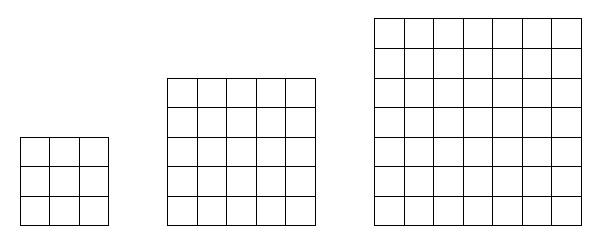
\includegraphics{energy-dp-grid-size.eps}
  \caption{The two-dimensional search space of possible positions on a 
    $m \times m$ sized grid, where $m$ is 3, 5, and 7.}
  \label{fig:energy-dp-grid-size}
\end{figure}

To find a global solution for a contour with minimum energy a backward
method is used which use a decision set that includes adjacent points
(see figure~\ref{fig:energy-dp-decision-set}). Usage of the adjacent
points are the reason why the computational complexity is
$\mathcal{O}(nm^3)$.
\begin{figure}[htbp]
  \centering
  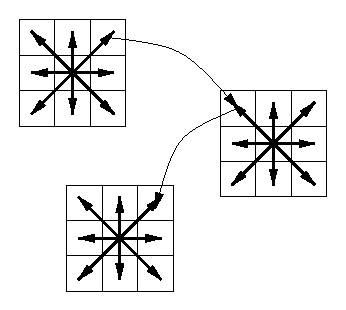
\includegraphics[]{energy-dp-decision-set.eps}
  \caption{The decision set for the dynamic programming energy
    minimization method for a single point with a minimum search space
    $m~=~9$. The curved arrows indicate positions of a point for the
    contour with lower energy.}
  \label{fig:energy-dp-decision-set}
\end{figure}
Dynamic programming address problems of the traditional snake method
using variational calculus, which is numerical stability, convergence,
and global solution. The reason is mainly that the method finds a
solution from a global search space, and not an iterative procedure.
It is achieved with the expense being computationally demanding, which
can be a disadvantage for some applications.

\subsubsection{Greedy Algorithm}
\label{sec:greedy-algorithm}


Along the lines of dynamic programming another energy minimization
scheme is defined. The greedy algorithm is proposed by
\citet{williams90} and refined by \citet{yan94} and \citet{yan97}. The
method is based on dynamic programming and allow for hard constraints,
but uses local search space instead of finding a global path. The
computational complexity of the greedy algorithm is $\mathcal{O}(nm)$,
where the method retains the numerical stability and flexibility for
dynamic programming while being more than an order of magnitude
faster.

The greedy algorithm uses the same search space (see
figure~\ref{fig:energy-dp-grid-size}), but each node is moved by the
algorithm based only on a local consideration. The energy function of
the greedy algorithm uses finite differences. Central to the method is
the greedy algorithm for finding a local energy minima, which
essentially does two things. One part of the algorithm finds a local
energy minima, and the other part will eventually introduce corners by
lowering the $\beta$ value at specific parts of the contour by
considering thresholds for contour curvature and the gradient magnitude of the
external energy and properties of neighboring nodes.

Compared with the dynamic programming method the greedy tube algorithm
only finds a minimum energy within the local search space. By only
considering the local search space of a snake control points the
computational complexity is thus reduced compared to dynamic
programming. The reduction results in a computational complexity of
$\mathcal{O}(nm)$, where only the decision set of the local search
space of $n$ snake control points are evaluated (see
figure~\ref{fig:energy-greedy-decision-set}).
\begin{figure}[htbp]
  \centering
  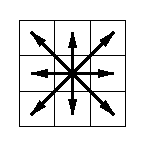
\includegraphics{energy-greedy-decision-set.eps}
  \caption{The decision set of the search space for a snake control point using the greedy algorithm.}
  \label{fig:energy-greedy-decision-set}
\end{figure}

The greedy algorithm retains the same disadvantages identified with
FDM and dynamic programming, which is the discretization and
approximation of derivatives. The algorithm compensates for this by
enforcing hard constraints on the minimum distance between nodes.



\subsubsection{B-snakes}
\label{sec:b-snakes}

Another energy minimization method is called B-snakes was proposed by
\citet{menet90} and \citet{liao92}. The contour is approximated by
parametric B-splines. The energy of the snake is computed by inserting
the approximated contour into the energy function. In this respect the
B-snakes is similar to FEM snakes. Between nodes the a segment is
approximated by $m~-~2$ segments and $m~-~1$ control knots. Each
segment of the contour is approximated by a piecewise polynomial
function $Q_i(s)$ of the order $k$ to be $k~-~1$ differentiable. The
piecewise polynomial function is a combination of basis functions
$B_i$ and control vertices $V_i = (x_i, y_i)$
\begin{equation}
  \nonumber
  Q_i(s) = \sum^m_{i=0} V_i B_i(s)
\end{equation}
Using B-splines gives the possibility to locally modify a segment
without affecting the rest of the contour. The solution is found by
approximating the contour by B-splines and writing the equations on
matrix form, finding the minima is similar fashion as FEM and FDM.

Advantages of using B-snakes are the possibility of local control of
segments without interfering with the rest of the contour. With a
differentiable contour, control knots of the contour can be placed on
top of each other to introduce corners on the contour. Disadvantages
is that approximation by B-splines the contour will not pass through
nodes, also by B-spline approximation the contour may not be located
at control knots. When inserting and removing control knots there is no
correspondence between old and new contour.

\subsubsection{Geometric Algorithms}
\label{sec:geometric-algorithms}

Two types of geometric energy minimization algorithms exist: the
geodesic level set approach and the other type that use true geometry
aspects to minimize the energy of a contour. The latter is used by
\citet{williams97} and defined in \citep{lobregt95}. The geometrical
aspect is used to compute contour normals at discrete points on the
contour. Deformation of the contour will happen on the basis of the
computed contour normals (see
figure~\ref{fig:energy-geometric-aspect}).
\begin{figure}[htbp]
  \centering
  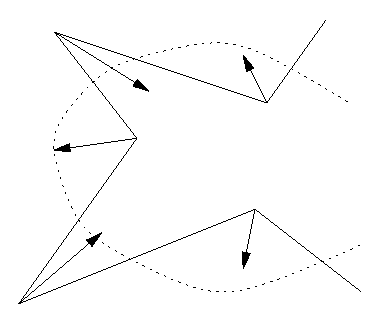
\includegraphics{energy-geometric-aspect.eps}
  \caption{The objective is to minimize the local contour curvature with geometric aspects}
  \label{fig:energy-geometric-aspect}
\end{figure}


The geometric  algorithms will find  an energy minima through  a level
set    (also   referred    to   as    front    propagation)   approach
\citep{osher88,malladi95,lorigo98,wang98,wang98b}.   A boundary  in an
image is found  by inserting the surface one  extra dimension into the
image (see  figure~\ref{fig:energy-level-set-approach}).  Evolution of
the boundary is  dependent upon the time and  location of surface with
respect to  the image  plane. The boundary  itself is  the zero-valued
contour  of $\phi$.  As  the front  of the  surface evolves  over time
$\phi$ is a function of space and time, where the evolution is defined
as
\begin{equation}
  \nonumber
  \phi_t(x(t), t) + F \lvert \nabla\phi(x(t), t) \rvert
\end{equation}
\begin{figure}[htbp]
  \centering
  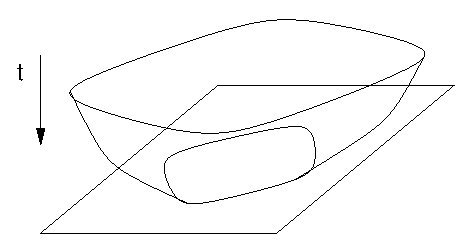
\includegraphics{energy-level-set-approach.eps}
  \caption{Level set approach where the surface of a higher dimension
    is inserted into the image plane, where the intersection of the
    surface and the image defines the contour boundary}
  \label{fig:energy-level-set-approach}
\end{figure}
The velocity function $F$ of the surface represents the speed of the
boundary motion and the initial condition is the location of the
insertion of the surface at $t~=~0$. It is through $F$ that the front
evolution of the boundary can be controlled. The function $F$ is split
into $F = F_A + F_G$, where $F_A$ is referred to as the advection term
which independently of the boundary contour expands or contracts the
boundary depending on the sign of $F_A$ (similar in nature as the
balloon energy). $F_G$ is the part which is dependent on the geometry
of the front which smoothes parts of the boundary contour with high
curvature and regularizing the contour (identical to the internal
energy term of traditional snakes). In this respect the method
resembles topological adaptable snakes.

The advantage is that the method make no assumptions of the topology
of the objects to segment, as the surface may split and join to
segment several objects simultaneously. 


\section{Evaluation of Methods}
\label{sec:evaluation-methods}

The representation of traditional deformable model methods are often
either open or closed two-dimensional contours or general
three-dimensional surfaces.  In this project a compact representation
will be used similar to those presented in
section~\ref{sec:models-thin-elong}, which are thin elongated
structures, a specific three-dimensional surface.  The contour
representation used, a generalized tube, have the following properties
\begin{itemize}
\item The representation consists of a central axis, referred to as
  the central axis, and a circular cross section swept along the central axis.
\item The circular cross section may vary its radius and may have radial
  displacements of the circular cross section contour.
\item The surface of the generalized tube is the contours of the swept
  cross section contours.
\end{itemize}
The  compact  representation  provides  both  a  generalized  cylinder
surface  and a central  axis for  the generalized  cylinders.  General
three-dimensional  surfaces are  normally  defined a  mesh of  surface
nodes. The advantages of the  general surfaces is that they may attain
any shape  at the  cost of a  very general definition.  Establishing a
central axis for an axis and cross section contours have to be derived
from the general surface representation.


The contour representation will reflect the deformable model that will extract
the surface model. Several issues must be decided upon when choosing
an representation
\begin{itemize}
\item Generality contrasted by specificity where a decision has to be
  made whether the deformable model must represent a broad range of
  shapes, with many different applications where the deformable model
  may come to use. Full automation may require a very specific model
  if the shape is known through \emph{a priori} knowledge, where task
  is to fit the model to data.
\item Compact model representation, geometric coverage, and
  topological flexibility are areas to consider when a model and its
  representation is chosen. Parametrized models offer explicit
  definition of surface while implicit models typically have greater
  topological variety.
\end{itemize}


Energy definition of internal, external, and constraints are almost
all defined in the two-dimensional context. Most are easily applied to
contours with a co-dimension of one (see
section~\ref{sec:snake-representation}). Extension to contours with a
co-dimension of two may have the energy definitions extended to be
parametrized by two variables~$s$ and~$t$. More specific models like
the class of generalized cylinders need to have other additional
energies defined to make contour converge to image features. The
energy definition, the contour representation and the energy
minimization methods are dependent upon each other. The energy
function definition is the link between the contour representation and
the energy minimization method. The energy function will include
internal and external energies. Since the system to be created will be
automatic no interactive energies are considered.


The energy minimization methods can be divided into three groups. The
FDM, FEM and B-snakes methods have similar characteristics, dynamic
programming and greedy algorithm share the same fundamentals and 
geodesic and geometric methods being similar. General advantages and
disadvantages of these three groups will be indicated here along with
specific properties of each method. The advantages of the energy
minimization methods are
\begin{description}
\item[Continuous Curve] The Geodesic, FEM, and B-snakes method uses the
  information between the nodes. The continuous curve may have its 

\item[Simple Implementation] The FDM and the Greedy Algorithm are
  relatively simple to implement.

\item[Global Minimum] The dynamic programming method will from the
  search path find a global energy minimum of the contour.
\end{description}
The disadvantages of the methods are
\begin{description}
\item[Discrete Curve] FDM, dynamic programming and greedy algorithm
  only use the information at the nodes of the contour.

\item[No Global Minimum] The FDM, FEM, and B-snakes are not guaranteed
  to find a global minimum but may converge only to a local minimum.
  
\item[Numerical Instability] The FDM, FEM, and B-snakes use
  variational calculus which may introduce numerical instability. This
  is due to problems with non-uniform distances between contour nodes,
  when finding derivatives and numerical instability, that is
  introduced through the iterative solution routines.

\item[Many Contour Nodes] To segment a high degree of details on the
  contour the contour must be sampled by many control nodes, which
  lead to greater computation demands.
\end{description}
To some extent the reviewed energy minimization methods use the same
energy function definition but use different approaches for finding a
minimum energy. Used with a generalized cylinder and an extended
energy function defined for a generalized cylinder these methods
cannot be used ``as is'' but must be extended to meet the demands of
the representation and the energy function definition. This is true
for both general three-dimensional and tube surface representations.




\clearemptydoublepage

%%% Local Variables: 
%%% mode: latex
%%% mode: reftex
%%% mode: flyspell
%%% TeX-master: "master"
%%% End: 
